\section{AQSE Framework}
\label{sec:framework}

AQSE separates acquisition, feature construction, quantum representation, and classical prediction. Figure~\ref{fig:aqse-routes} distinguishes the network demonstrator from the component-level benchmark. Both use the same eight-qubit circuit and fidelity kernel. Their feature profiles, training populations, and prediction interfaces differ. The definitions below describe the implementation frozen with the canonical study records~\cite{aqse2026canonical}.

\begin{figure*}[t]
\centering
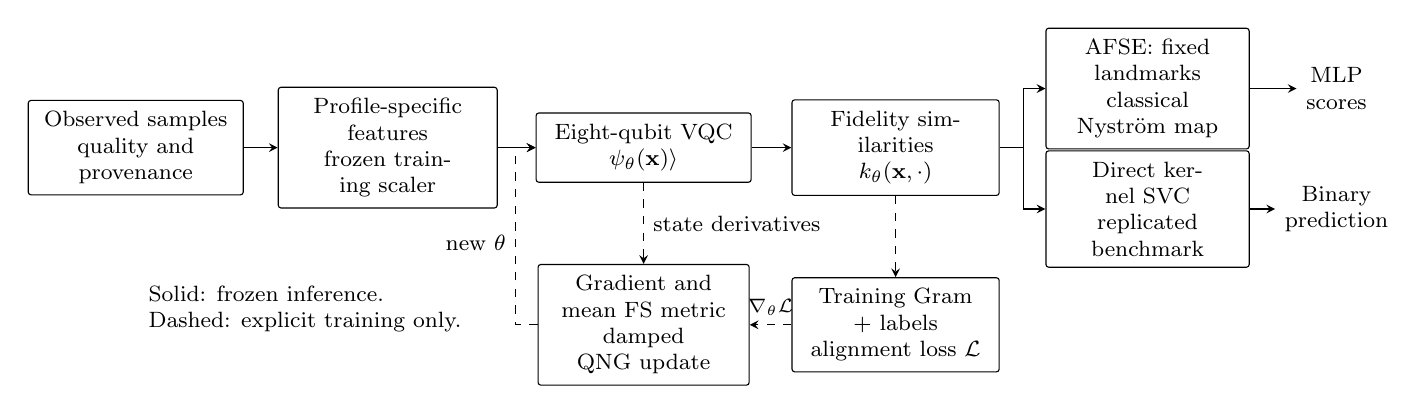
\begin{tikzpicture}[x=1cm,y=1cm,>=stealth,
  box/.style={draw,rounded corners=1pt,align=center,font=\footnotesize,inner sep=4pt,minimum height=0.82cm},
  small/.style={font=\footnotesize,align=center}]
\node[box,text width=2.45cm] (obs) at (0,0) {Observed samples\\quality and provenance};
\node[box,text width=2.50cm] (feat) at (3.20,0) {Profile-specific features\\frozen training scaler};
\node[box,text width=2.45cm] (state) at (6.45,0) {Eight-qubit VQC\\$\lvert\psi_{\boldsymbol\theta}(\mathbf x)\rangle$};
\node[box,text width=2.35cm] (kernel) at (9.65,0) {Fidelity similarities\\$k_{\boldsymbol\theta}(\mathbf x,\cdot)$};
\draw[->] (obs)--(feat); \draw[->] (feat)--(state); \draw[->] (state)--(kernel);
\node[box,text width=2.3cm] (afse) at (12.85,0.75) {AFSE: fixed landmarks\\classical Nystr\"om map};
\node[box,text width=2.3cm] (svm) at (12.85,-0.78) {Direct kernel SVC\\replicated benchmark};
\draw[->] (kernel.east) -- ++(0.30,0) |- (afse.west);
\draw[->] (kernel.east) -- ++(0.30,0) |- (svm.west);
\node[small] (mlp) at (15.25,0.75) {MLP\\scores};
\node[small] (binary) at (15.25,-0.78) {Binary\\prediction};
\draw[->] (afse.east)--(mlp.west); \draw[->] (svm.east)--(binary.west);
\node[box,text width=2.35cm] (loss) at (9.65,-2.25) {Training Gram + labels\\alignment loss $\mathcal L$};
\node[box,text width=2.4cm] (qng) at (6.45,-2.25) {Gradient and mean FS metric\\damped QNG update};
\draw[->,dashed] (kernel.south)--(loss.north);
\draw[->,dashed] (loss.west)-- node[above,font=\scriptsize] {$\nabla_{\boldsymbol\theta}\mathcal L$} (qng.east);
\draw[->,dashed] (state.south)-- node[right,font=\footnotesize] {state derivatives} (qng.north);
\draw[->,dashed] (qng.west)-- ++(-0.28,0) |- node[pos=0.23,left,font=\footnotesize] {new $\boldsymbol\theta$} (state.west);
\node[small,align=left] at (2.15,-2.05) {Solid: frozen inference.\\Dashed: explicit training only.};
\end{tikzpicture}
\caption{AQSE processing boundaries. The network demonstrator uses State8 and the AFSE--MLP branch. The 30-replica experiment uses harmonic features and the direct-kernel SVC branch. Labels enter the training objective, not the observed feature vector. The mean Fubini--Study (FS) metric is computed from state derivatives, separately from the loss gradient. No simulator truth enters inference.}
\label{fig:aqse-routes}
\end{figure*}


\subsection{Observations and Feature Profiles}
\label{sec:framework-observations}

A simulated network contains $N_s\in\{1,\ldots,8\}$ nodes. Each vector reading includes three measured field components, a timestamp, observed temperature, orientation, calibration identity, and quality flags. Simulator truth is retained separately. It may define experimental labels but is not an input to the feature extractor or predictor. The number of nodes is independent of the eight input coordinates and eight qubits. A circuit represents one accepted feature vector, not one qubit per sensor.

The demonstrator uses \emph{State8}, with separate local and network profiles. Let $R_i[k]$ map world-frame vectors to the sensor frame. The observed world-North component is
\begin{equation}
 b_i[k]=\mathbf e_N^{\mathsf T}R_i[k]^{\mathsf T}
             \mathbf B_i^{\mathrm{obs}}[k],
 \label{eq:north-observation}
\end{equation}
converted to nanotesla before feature extraction. This rotation uses the declared orientation. It does not infer or correct an unknown calibration error. At 100~Hz, an initial 800-sample reference freezes the mean North field $\bar b_{i,0}$ and temperature $\bar T_{i,0}$. Subsequent 400-sample windows advance by 100 samples. Within a window, define $d_i[k]=b_i[k]-\bar b_{i,0}$, with $k=0,\ldots,399$. Table~\ref{tab:state8} specifies the coordinates. Each accepted window uses only measurements acquired by its endpoint.

\begin{table}[t]
\caption{State8 coordinates in the network demonstrator. The local and network profiles share $x_0$--$x_4$ and $x_7$.}
\label{tab:state8}
\centering
\footnotesize
\setlength{\tabcolsep}{3pt}
\renewcommand{\arraystretch}{1.15}
\begin{tabular}{@{}cll@{}}
\toprule
Index & Definition & Unit\\
\midrule
$x_0$ & $\operatorname{mean}_k d_i[k]$ & nT\\
$x_1$ & $1.4826\operatorname{median}_k|d_i[k]-\operatorname{median}d_i|$ & nT\\
$x_2$ & Least-squares slope of $d_i[k]$ versus time & nT/s\\
$x_3$ & $10\log_{10}(\max(P_L,\epsilon)/\max(P_H,\epsilon))$ & dB\\
$x_4$ & $\operatorname{mean}_k T_i[k]-\bar T_{i,0}$ & K\\
\midrule
\multicolumn{3}{@{}l}{Local profile}\\
$x_5$ & $\sqrt{\operatorname{mean}_k(d_i[k+1]-d_i[k])^2}$ & nT\\
$x_6$ & $\operatorname{corr}(d_i[0{:}399],d_i[1{:}400])$ & 1\\
\midrule
\multicolumn{3}{@{}l}{Network profile}\\
$x_5$ & $\sqrt{\operatorname{mean}_k(d_i[k]-\operatorname{median}_{j\in\mathcal P_i}d_j[k])^2}$ & nT\\
$x_6$ & $|\mathcal P_i|^{-1}\sum_{j\in\mathcal P_i}\operatorname{corr}(d_i,d_j)$ & 1\\
\midrule
$x_7$ & Received vector samples / 400 & 1\\
\bottomrule
\end{tabular}
\par\smallskip
\begin{minipage}{\columnwidth}\footnotesize
$P_L$ and $P_H$ integrate a linearly detrended, Hann-windowed one-sided periodogram over $[0.25,2)$ and $[2,20]$~Hz. The power floor is $\epsilon=10^{-12}$~nT$^2$. Correlations are Pearson coefficients. Slice endpoints are exclusive.
\end{minipage}
\end{table}


For the network profile, the peer set $\mathcal P_i$ contains at least two other nodes with complete, aligned windows and valid references. With fewer valid peers, the runtime uses the compatible local path or abstains. One or two nodes do not support the network attribution task. Missing, stuck, clipped, or temporally inconsistent readings are not replaced by valid zeros. Undefined correlations also prevent the corresponding profile from entering inference. Under the implemented complete-window eligibility policy, the received fraction $x_7$ equals one for accepted windows; it remains informative in the quality record of rejected windows. An initial reference defines a measured baseline, not a certified normal state.

The replicated benchmark uses a different, harmonic feature vector,
\begin{equation}
 \mathbf x^{\mathrm{harm}}=
 (A,\phi,f,v,d,\mathrm{SNR},P_{\mathrm{peak}},T)^{\mathsf T},
 \label{eq:harmonic-vector}
\end{equation}
whose entries are oscillation amplitude, phase, frequency, variance, drift, signal-to-noise ratio, peak power spectral density (nT$^2$/Hz), and temperature. These are the extractor's fixed coordinates, not State8 coordinates. Each simulated episode contributes one predetermined window. The experiment therefore tests noise-regime classification through a direct kernel SVC. It does not measure the network demonstrator's causal attribution or AFSE classifier performance.

\subsection{Training-Only Scaling and Angle Encoding}
\label{sec:framework-encoding}

For each coordinate $j$, the shared \texttt{AngleScaler} stores the training mean $\mu_j$ and population standard deviation $\sigma_j$. It sets $s_j=\sigma_j$ when $\sigma_j>10^{-12}$ and $s_j=1$ otherwise. Its bounded map is
\begin{equation}
 a_j(\mathbf x)=\frac{\pi}{2}
    \tanh\!\left(\frac{x_j-\mu_j}{2s_j}\right),
 \qquad j=0,\ldots,7.
 \label{eq:angle-scaler}
\end{equation}
State8 uses~\eqref{eq:angle-scaler} on all eight coordinates. The harmonic benchmark instead replaces its phase coordinate by
\begin{equation}
 a_1(\mathbf x^{\mathrm{harm}})
   =\operatorname{wrap}_{[-\pi,\pi)}(\phi)
   =((\phi+\pi)\bmod 2\pi)-\pi.
 \label{eq:phase-direct}
\end{equation}
The other seven outputs remain unchanged. This convention respects phase periodicity but does not establish a common clock or cross-sensor phase reference. The harmonic phase is relative to the start of its window. Scaler parameters are fitted once on the relevant training population and remain fixed for validation, test, and subsequent queries. Neither query batching nor landmark selection refits them. The two encoding policies define different input spaces and are not interchangeable.

\subsection{Variational Circuit and Fidelity Kernel}
\label{sec:framework-kernel}

The circuit starts in $\lvert0\rangle^{\otimes8}$. Write its 16 parameters as $\boldsymbol\theta=(\boldsymbol\alpha,\boldsymbol\beta)$, where $\alpha_q=\theta_q$ and $\beta_q=\theta_{8+q}$. Define
\begin{equation}
 D_\nu(\mathbf a)=\bigotimes_{q=0}^{7}R_\nu(a_q),
 \qquad
 V_\nu(\boldsymbol\gamma)=\bigotimes_{q=0}^{7}R_\nu(\gamma_q),
 \label{eq:circuit-layers}
\end{equation}
for $\nu\in\{y,z\}$. With operators acting from right to left,
\begin{align}
 U_{\boldsymbol\theta}(\mathbf a)
  &=D_z(\mathbf a)V_y(\boldsymbol\beta)E
                  V_z(\boldsymbol\alpha)D_y(\mathbf a),
 \label{eq:vqc-unitary}\\
 \lvert\psi_{\boldsymbol\theta}(\mathbf x)\rangle
  &=U_{\boldsymbol\theta}(\mathbf a(\mathbf x))
                         \lvert0\rangle^{\otimes8}.
 \label{eq:encoded-state}
\end{align}
The entangler $E$ applies the even CZ edges $(0,1)$, $(2,3)$, $(4,5)$, and $(6,7)$ first, followed by $(1,2)$, $(3,4)$, and $(5,6)$. The graph is a path, not a ring. Figure~\ref{fig:tqk8-circuit} gives the gate sequence. A state preparation contains 32 single-qubit rotations and seven CZ gates. Every input angle appears twice; every trainable parameter appears once.

\begin{figure*}[t]
\centering
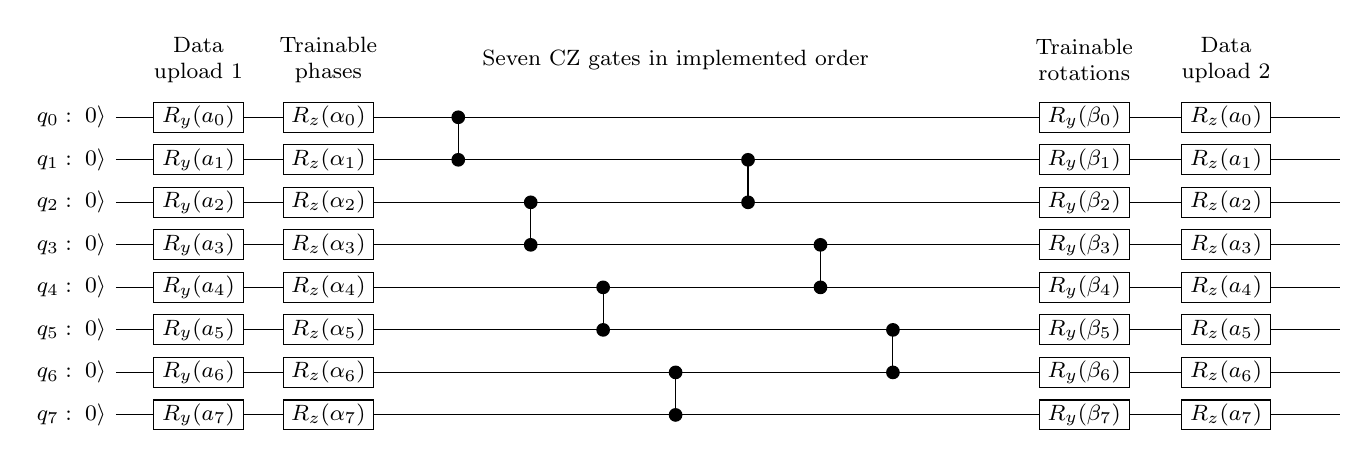
\begin{tikzpicture}[x=1cm,y=0.54cm,gate/.style={draw,fill=white,minimum width=1.14cm,minimum height=0.38cm,inner sep=1pt,font=\footnotesize},dot/.style={circle,fill,inner sep=1.75pt}]
\draw (0,0) -- (15.55,0);
\node[left,font=\footnotesize] at (0,0) {$q_0:\;\lvert0\rangle$};
\node[gate] at (1.05,0) {$R_y(a_0)$};
\node[gate] at (2.7,0) {$R_z(\alpha_0)$};
\node[gate] at (12.30,0) {$R_y(\beta_0)$};
\node[gate] at (14.10,0) {$R_z(a_0)$};
\draw (0,-1) -- (15.55,-1);
\node[left,font=\footnotesize] at (0,-1) {$q_1:\;\lvert0\rangle$};
\node[gate] at (1.05,-1) {$R_y(a_1)$};
\node[gate] at (2.7,-1) {$R_z(\alpha_1)$};
\node[gate] at (12.30,-1) {$R_y(\beta_1)$};
\node[gate] at (14.10,-1) {$R_z(a_1)$};
\draw (0,-2) -- (15.55,-2);
\node[left,font=\footnotesize] at (0,-2) {$q_2:\;\lvert0\rangle$};
\node[gate] at (1.05,-2) {$R_y(a_2)$};
\node[gate] at (2.7,-2) {$R_z(\alpha_2)$};
\node[gate] at (12.30,-2) {$R_y(\beta_2)$};
\node[gate] at (14.10,-2) {$R_z(a_2)$};
\draw (0,-3) -- (15.55,-3);
\node[left,font=\footnotesize] at (0,-3) {$q_3:\;\lvert0\rangle$};
\node[gate] at (1.05,-3) {$R_y(a_3)$};
\node[gate] at (2.7,-3) {$R_z(\alpha_3)$};
\node[gate] at (12.30,-3) {$R_y(\beta_3)$};
\node[gate] at (14.10,-3) {$R_z(a_3)$};
\draw (0,-4) -- (15.55,-4);
\node[left,font=\footnotesize] at (0,-4) {$q_4:\;\lvert0\rangle$};
\node[gate] at (1.05,-4) {$R_y(a_4)$};
\node[gate] at (2.7,-4) {$R_z(\alpha_4)$};
\node[gate] at (12.30,-4) {$R_y(\beta_4)$};
\node[gate] at (14.10,-4) {$R_z(a_4)$};
\draw (0,-5) -- (15.55,-5);
\node[left,font=\footnotesize] at (0,-5) {$q_5:\;\lvert0\rangle$};
\node[gate] at (1.05,-5) {$R_y(a_5)$};
\node[gate] at (2.7,-5) {$R_z(\alpha_5)$};
\node[gate] at (12.30,-5) {$R_y(\beta_5)$};
\node[gate] at (14.10,-5) {$R_z(a_5)$};
\draw (0,-6) -- (15.55,-6);
\node[left,font=\footnotesize] at (0,-6) {$q_6:\;\lvert0\rangle$};
\node[gate] at (1.05,-6) {$R_y(a_6)$};
\node[gate] at (2.7,-6) {$R_z(\alpha_6)$};
\node[gate] at (12.30,-6) {$R_y(\beta_6)$};
\node[gate] at (14.10,-6) {$R_z(a_6)$};
\draw (0,-7) -- (15.55,-7);
\node[left,font=\footnotesize] at (0,-7) {$q_7:\;\lvert0\rangle$};
\node[gate] at (1.05,-7) {$R_y(a_7)$};
\node[gate] at (2.7,-7) {$R_z(\alpha_7)$};
\node[gate] at (12.30,-7) {$R_y(\beta_7)$};
\node[gate] at (14.10,-7) {$R_z(a_7)$};
\draw (4.35,0) -- (4.35,-1);
\node[dot] at (4.35,0) {};
\node[dot] at (4.35,-1) {};
\draw (5.27,-2) -- (5.27,-3);
\node[dot] at (5.27,-2) {};
\node[dot] at (5.27,-3) {};
\draw (6.19,-4) -- (6.19,-5);
\node[dot] at (6.19,-4) {};
\node[dot] at (6.19,-5) {};
\draw (7.11,-6) -- (7.11,-7);
\node[dot] at (7.11,-6) {};
\node[dot] at (7.11,-7) {};
\draw (8.03,-1) -- (8.03,-2);
\node[dot] at (8.03,-1) {};
\node[dot] at (8.03,-2) {};
\draw (8.95,-3) -- (8.95,-4);
\node[dot] at (8.95,-3) {};
\node[dot] at (8.95,-4) {};
\draw (9.87,-5) -- (9.87,-6);
\node[dot] at (9.87,-5) {};
\node[dot] at (9.87,-6) {};
\node[font=\footnotesize,align=center] at (1.05,1.35) {Data\\upload 1};
\node[font=\footnotesize,align=center] at (2.7,1.35) {Trainable\\phases};
\node[font=\footnotesize] at (7.11,1.35) {Seven CZ gates in implemented order};
\node[font=\footnotesize,align=center] at (12.30,1.35) {Trainable\\rotations};
\node[font=\footnotesize,align=center] at (14.10,1.35) {Data\\upload 2};
\end{tikzpicture}
\caption{Protected TQK8 state-preparation circuit, read from left to right. Here $a_q$ is an encoded feature, $\alpha_q=\theta_q$, and $\beta_q=\theta_{8+q}$. A line with two filled endpoints denotes CZ. The seven gates are drawn sequentially to preserve the source order; no hardware schedule or transpiled depth is implied. The circuit has no measurement in exact-state evaluation.}
\label{fig:tqk8-circuit}
\end{figure*}


The shared-parameter fidelity kernel in~\eqref{eq:fidelity-kernel} can also be written as
\begin{equation}
 k_{\boldsymbol\theta}(\mathbf x,\mathbf x')=
 \operatorname{Tr}\!\left[\rho_{\boldsymbol\theta}(\mathbf x)
                           \rho_{\boldsymbol\theta}(\mathbf x')\right],
 \label{eq:density-kernel}
\end{equation}
where $\rho_{\boldsymbol\theta}(\mathbf x)=\lvert\psi_{\boldsymbol\theta}(\mathbf x)\rangle\langle\psi_{\boldsymbol\theta}(\mathbf x)\rvert$. This Hilbert--Schmidt inner product establishes positive semidefiniteness~\cite{schuld2019feature,havlicek2019supervised}. Exact normalized states give $k(\mathbf x,\mathbf x)=1$ and $0\leq k\leq1$. The final data-dependent layer in~\eqref{eq:vqc-unitary} prevents the circuit from reducing to a feature map followed solely by a common trainable unitary. Such a terminal unitary would cancel from the overlap and could not train the kernel.

The implementation provides independent NumPy and Qiskit statevector engines. The replicated study uses NumPy exact-state evaluation, without shots, hardware noise, or QPU submission. An ancilla-free overlap circuit is also defined: prepare $U_{\boldsymbol\theta}(\mathbf a)$, apply $U_{\boldsymbol\theta}(\mathbf a')^\dagger$, and measure the all-zero probability. Its existence is not evidence of a hardware experiment. The direct binary kernel classifier has decision function
\begin{equation}
 f(\mathbf x)=\sum_{i\in\mathcal S}c_i y_i
                k_{\boldsymbol\theta}(\mathbf x_i,\mathbf x)+b,
 \label{eq:kernel-svc}
\end{equation}
where $\mathcal S$ indexes the fitted support vectors. In the replicated benchmark, circuit optimization uses 32 balanced training examples, whereas the SVC uses all 72 training examples.

\subsection{Alignment Objective and Quantum Natural Gradient}
\label{sec:framework-qng}

For a binary training bank of size $M$, let $K_{\boldsymbol\theta}$ be its Gram matrix, $\mathbf y\in\{-1,+1\}^{M}$ its target vector, and $H=I_M-\mathbf1\mathbf1^{\mathsf T}/M$. The implemented objective is one minus centered kernel--target alignment~\cite{cortes2012alignment,hubregtsen2022training}:
\begin{align}
 K_c&=HK_{\boldsymbol\theta}H,
 &Y_c&=(H\mathbf y)(H\mathbf y)^{\mathsf T},\nonumber\\
 \mathcal L(\boldsymbol\theta)
   &=1-\frac{\langle K_c,Y_c\rangle_F}
                 {\|K_c\|_F\,\|Y_c\|_F}.
 \label{eq:alignment-loss}
\end{align}
The implementation rejects a centered kernel or target norm below $10^{-12}$. Labels enter this objective, not the observation vector. The loss is a training surrogate. It is not the SVC objective or a held-out accuracy measure.

Because each parameter occurs once in a Pauli rotation, the state derivative used by the exact simulator is
\begin{equation}
 \partial_r\lvert\psi_{\boldsymbol\theta}(\mathbf x)\rangle
 =\frac{
 \lvert\psi_{\boldsymbol\theta+\frac{\pi}{2}\mathbf e_r}(\mathbf x)\rangle
 -\lvert\psi_{\boldsymbol\theta-\frac{\pi}{2}\mathbf e_r}(\mathbf x)\rangle}
 {2\sqrt{2}}.
 \label{eq:state-derivative}
\end{equation}
This is an amplitude derivative, not the usual probability-shift formula. If $o_{ij}=\langle\psi_i\mid\psi_j\rangle$, then
\begin{equation}
 \partial_r K_{ij}=2\operatorname{Re}\!\left[
 o_{ij}^{*}\big(\langle\partial_r\psi_i\mid\psi_j\rangle
          +\langle\psi_i\mid\partial_r\psi_j\rangle\big)\right].
 \label{eq:kernel-derivative}
\end{equation}
Both occurrences of the shared parameter contribute to the gradient.

AQSE uses the empirical mean Fubini--Study metric~\cite{stokes2020qng}:
\begin{equation}
 \bar g_{rs}=\frac{1}{M}\sum_{i=1}^{M}\operatorname{Re}\!\left[
 \langle\partial_r\psi_i\mid\partial_s\psi_i\rangle
 -\langle\partial_r\psi_i\mid\psi_i\rangle
  \langle\psi_i\mid\partial_s\psi_i\rangle\right].
 \label{eq:mean-fs}
\end{equation}
No factor of four is applied. The implementation forms the full $16\times16$ matrix, then symmetrizes it numerically. This is a chosen state-space preconditioner. It is not asserted to be the unique natural metric of the kernel matrix or classifier.

Let $\mathbf h=\nabla_{\boldsymbol\theta}\mathcal L$. A tentative step is
\begin{align}
 \mathbf v&=\eta(\bar g+\lambda_g I_{16})^{-1}\mathbf h,\nonumber\\
 \boldsymbol\delta&=\min\!\left(1,\frac{\delta_{\max}}{\|\mathbf v\|_2}\right)
                 \mathbf v,
 \label{eq:damped-qng}
\end{align}
with $\eta=0.2$, $\lambda_g=10^{-3}$, and $\delta_{\max}=0.4$. A candidate $\boldsymbol\theta-\boldsymbol\delta$ is accepted only if
\begin{equation}
 \mathcal L(\boldsymbol\theta-\boldsymbol\delta)
 \leq\mathcal L(\boldsymbol\theta)-10^{-4}
                       \mathbf h^{\mathsf T}\boldsymbol\delta.
 \label{eq:armijo-qng}
\end{equation}
The step is halved after rejection, with at most 12 candidate evaluations per update. A gradient norm below $10^{-10}$ or failure to accept a step stops optimization. The study permits at most ten accepted updates and preserves the initial checkpoint. Optimizer coordinates are not wrapped or clamped after an update.

The target is task-specific. The harmonic study uses nominal versus elevated noise labels. The demonstrator's local loss uses normal versus change labels. Its network loss uses only environment-compatible versus device-compatible training examples. Normal and mixed examples are excluded from that binary optimization bank but remain available to the downstream four-class model. Thus, network QNG does not directly optimize the four-class prediction loss.

\subsection{Fixed-Landmark AFSE Representation}
\label{sec:framework-afse}

The demonstrator converts kernel similarities into a fixed-dimensional vector using a regularized Nystr\"om map~\cite{williams2001nystrom}. AQSE calls this interface AFSE. It is a classical transformation of quantum-kernel evaluations, not a second quantum circuit.

Let $\mathcal Z=(\mathbf z_1,\ldots,\mathbf z_m)$ be an ordered, class-balanced set of training landmarks, with one distinct generative lineage per landmark. The requested size is 32. If training support is insufficient, the implementation reduces $m$ while retaining class balance; the output dimension then equals the recorded $m\leq32$. Landmark identities, order, encoding, and $\boldsymbol\theta$ are frozen together. Define
\begin{align}
 W_{ij}&=k_{\boldsymbol\theta}(\mathbf z_i,\mathbf z_j),
 &\mathbf k_{\mathcal Z}(\mathbf x)_j
    &=k_{\boldsymbol\theta}(\mathbf x,\mathbf z_j),\nonumber\\
 W&=Q\operatorname{diag}(\boldsymbol\lambda)Q^{\mathsf T}.
 \label{eq:landmark-gram}
\end{align}
An eigenvalue below $-10^{-10}\max(1,\lambda_{\max})$ causes rejection. Smaller numerical negatives are clipped to zero, giving $\lambda_j^+=\max(\lambda_j,0)$. The stored symmetric inverse square root is
\begin{equation}
 B=Q\operatorname{diag}\!\left((\lambda_j^++\lambda_N)^{-1/2}\right)
       Q^{\mathsf T},\qquad \lambda_N=10^{-6}.
 \label{eq:nystrom-basis}
\end{equation}
The column-vector embedding and its induced approximate kernel are
\begin{align}
 \mathbf z(\mathbf x)&=B\mathbf k_{\mathcal Z}(\mathbf x),
 \label{eq:afse-map}\\
 \widetilde k(\mathbf x,\mathbf x')
   &=\mathbf k_{\mathcal Z}(\mathbf x)^{\mathsf T}B^2
                              \mathbf k_{\mathcal Z}(\mathbf x').
 \label{eq:afse-kernel}
\end{align}
For row-oriented batches, the implementation evaluates $K_{X\mathcal Z}B$. A query's coordinates depend on the frozen representation, not on other queries in the batch. The regularization and finite landmark set mean that $\widetilde k$ need not equal $k_{\boldsymbol\theta}$.

The diagnostic residual is
\begin{equation}
 r(\mathbf x)=k_{\boldsymbol\theta}(\mathbf x,\mathbf x)
                    -\|\mathbf z(\mathbf x)\|_2^2.
 \label{eq:afse-residual}
\end{equation}
Values below $-10^{-10}$ are rejected; smaller numerical negatives are set to zero. The runtime flags a query when its residual exceeds the empirical training 99th percentile. This is a reference-coverage heuristic. It is neither a calibrated out-of-distribution test nor evidence of a physical fault. Training landmarks are included in the population used to set that threshold. AFSE is absent from the replicated direct-kernel benchmark.

\subsection{Classical Output and Runtime Boundaries}
\label{sec:framework-runtime}

The demonstrator standardizes AFSE vectors using training statistics and fits a multilayer perceptron with hidden widths 32 and 16. With standardized input $\widehat{\mathbf z}$, its logits are
\begin{equation}
 \mathbf u=W_3\tanh\!\left(W_2\tanh(W_1\widehat{\mathbf z}+\mathbf b_1)
                  +\mathbf b_2\right)+\mathbf b_3.
 \label{eq:mlp-logits}
\end{equation}
Binary output uses a sigmoid; four-class output uses a softmax. Fitting uses L-BFGS and an $L_2$ regularization coefficient of $10^{-3}$. A raw-State8 baseline uses the same hidden widths with separately fitted training preprocessing. It has a different input dimension and is not parameter-count matched to the AFSE model. This baseline is also distinct from the 11-parameter MLP in the replicated experiment.

The local task reports normal or change. The network task reports normal, environment-compatible, device-compatible, or mixed/ambiguous patterns. These labels express similarity to simulated training conditions, not identified physical causes. A top score below 0.70 or a top-two score margin below 0.15 produces an uncertainty status. Quality failures and incompatible representations can instead cause abstention. Scores are not treated as calibrated probabilities.

A model bundle binds the feature profile, fitted scaler, encoding policy, exact circuit parameters, landmarks, AFSE basis, downstream standardizer, and classifier. Applying a different bundle invalidates cached representations and pending results from the previous one. Training is explicit and cancellable between optimizer calls. It does not run at every measurement or backend restart. Simulation time, data transport, and analysis cadence are separate. The inference worker uses a bounded buffer and a newest-window queue, reporting result age, skipped windows, and latency. These controls make the computation auditable; they do not establish real-time guarantees or field diagnostic accuracy.
